% !TeX program = xelatex
% !TeX encoding = UTF-8
% !TeX TXS-program:compile = txs:///xelatex | txs:///xelatex
\documentclass[aspectratio=169, table, 12pt]{beamer}

% Preamble bersama seluruh slide mata kuliah ini.
% Dipanggil dari slides/sessionXX/sessionXX.tex tepat sesudah baris
% \documentclass[aspectratio=169, table, 12pt]{beamer}
% Paket tambahan yang hanya dibutuhkan satu sesi ditulis di berkas sesi itu.

\usepackage{colortbl}
\usepackage{xcolor}
\usepackage{listings}
\usepackage{tabularx}
\usepackage{booktabs}
\usepackage{tikz}
\usepackage{pgfplots}
\usepackage{fontspec}
\usepackage[english,bahasai]{babel}
\pgfplotsset{compat=1.18}
\usetikzlibrary{arrows.meta, positioning, calc, fit, shapes.geometric,
  shapes.multipart, backgrounds, matrix, chains, trees}

\makeatletter
\def\input@path{{../theme/}}
\makeatother
\graphicspath{{../theme/}{../../figures/}}
% Stub symlink Windows memakai tema cadangan sampai aset institusi tersedia.
\IfFileExists{../theme/beamerthemePradita.sty}{%
  \usetheme{Pradita}
}{%
  \usetheme{Madrid}
  \setmainfont{TeX Gyre Heros}
  \setsansfont{TeX Gyre Heros}
  \setbeamertemplate{navigation symbols}{}
}

\definecolor{praditagreen}{RGB}{37, 113, 71}
\setbeamercolor{structure}{fg=praditagreen}
\setbeamercolor{palette primary}{bg=praditagreen,fg=white}
\setbeamercolor{palette secondary}{bg=praditagreen!80!black,fg=white}
\setbeamercolor{palette tertiary}{bg=praditagreen!60!black,fg=white}
\setbeamerfont{frametitle}{size=\large}
\setbeamertemplate{caption}[numbered]

% Ukuran header mengikuti teks agar judul panjang tidak menabrak logo.
\setbeamercolor{frametitle}{bg=white,fg=black}
\setbeamertemplate{frametitle}{%
  \begin{beamercolorbox}[wd=\paperwidth,sep=0.2cm]{frametitle}
    \begin{minipage}[c]{0.77\paperwidth}
      \raggedright\fontsize{16}{18}\selectfont\bfseries\insertframetitle
      \ifx\insertframesubtitle\empty\else
        \par\small\mdseries\insertframesubtitle
      \fi
    \end{minipage}\hfill
    \begin{minipage}[c]{0.15\paperwidth}
      \IfFileExists{../theme/classFiles/logo_universitas.png}{%
        
\includegraphics[width=\linewidth]{../theme/classFiles/logo_universitas.png}%
      }{}
    \end{minipage}
  \end{beamercolorbox}
}
\setbeamertemplate{footline}{%
  \ifnum\value{framenumber}>1
    \begin{beamercolorbox}[wd=\paperwidth,ht=0.35cm,dp=0.15cm,
      leftskip=0.3cm,rightskip=0.3cm]{palette primary}
      \footnotesize\bfseries\insertframenumber/\inserttotalframenumber
      \hfill IT40813
    \end{beamercolorbox}
  \fi
}
\DeclareRobustCommand{\berkas}[1]{\path{#1}}

% Tema membuat garis tabel berwarna putih. Dikembalikan agar tabel terbaca.
\arrayrulecolor{black}
\setlength{\arrayrulewidth}{0.5pt}

\lstdefinelanguage{yaml}{
  basicstyle=\ttfamily\scriptsize,
  keywordstyle=\color{blue}\bfseries,
  commentstyle=\color{gray}\itshape,
  stringstyle=\color{red},
  showstringspaces=false,
  breaklines=true,
  frame=lines,
  numbers=none,
  backgroundcolor=\color{lightgray!10},
  tabsize=2,
  morecomment=[l]{\#}
}

\lstdefinelanguage{json}{
  basicstyle=\ttfamily\scriptsize,
  stringstyle=\color{red},
  commentstyle=\color{gray},
  breaklines=true,
  showstringspaces=false,
  tabsize=2,
  numbers=none,
  frame=lines,
  backgroundcolor=\color{lightgray!10},
  string=[s]{"}{"}
}

\lstdefinelanguage{bash}{
  keywords={},
  basicstyle=\ttfamily\scriptsize,
  ndkeywords={docker, kubectl, helm, curl, git, terraform},
  ndkeywordstyle=\color{purple}\bfseries,
  sensitive=true,
  commentstyle=\color{gray},
  numbers=none,
  breaklines=true,
  frame=lines,
  backgroundcolor=\color{lightgray!10},
  tabsize=2,
  comment=[l]{\#},
  showstringspaces=false
}

\lstdefinelanguage{http}{
  keywords={GET, POST, PUT, PATCH, DELETE, HEAD, OPTIONS, HTTP},
  basicstyle=\ttfamily\scriptsize,
  keywordstyle=\color{blue}\bfseries,
  sensitive=true,
  numbers=none,
  breaklines=true,
  frame=lines,
  backgroundcolor=\color{lightgray!10},
  tabsize=2,
  showstringspaces=false
}

\subtitle{IT40813 · IT Governance, Risk \& Compliance}
\author{\textbf{Alfa Yohannis}}


% Sampul membatasi judul di panel putih tema rujukan Pradita.
\setbeamertemplate{title page}{%
  \begin{tikzpicture}[remember picture,overlay]
    \node[anchor=north west,inner sep=0pt,text width=8.8cm]
      at ([xshift=1cm,yshift=-3.15cm]current page.north west) {%
        {\small\insertsubtitle\par}\vspace{0.25cm}
        \resizebox{8.8cm}{!}{\begin{minipage}{12cm}
          \raggedright\color{praditagreen}\bfseries\inserttitle
        \end{minipage}}
      };
    \node[anchor=south west,inner sep=0pt]
      at ([xshift=1cm,yshift=1.65cm]current page.south west)
      {\small\insertdate};
    \node[anchor=west,inner sep=0pt,text=white]
      at ([xshift=0.8cm,yshift=0.75cm]current page.south west)
      {\small\insertauthor};
  \end{tikzpicture}
}


\title{\Huge KPI, KRI\\ \vspace{10pt} dan Pelaporan ke Direksi}
\date{Pertemuan 13}

\begin{document}

\frame{\titlepage}

\begin{frame}
  \frametitle{Isi Pertemuan}
  \vspace{14pt}
  \begin{columns}[t]
    \column{0.5\textwidth}
    {\small\tableofcontents[sections={1-5}]}

    \column{0.5\textwidth}
    {\small\tableofcontents[sections={6-9}]}
  \end{columns}
\end{frame}

\begin{frame}{\hfill}
  \centering
  \Huge{\textbf{Laporan 40 halaman\\sudah terbit.\\Keputusan apa yang diminta?}}
\end{frame}

\section{Tujuan dan Konteks}

\begin{frame}{{\Large Tujuan Pembelajaran}}
  \vspace{10pt}
  \begin{itemize}
    \item Membedakan KPI, KRI, dan KCI, lalu memilih indikator yang memicu tindakan.
    \item Menetapkan ambang batas KRI yang selaras dengan \textit{risk appetite}.
    \item Menyusun laporan GRC satu halaman yang dapat dipakai direksi untuk mengambil
          keputusan.
  \end{itemize}
\end{frame}

\begin{frame}{{\Large Masalah: Banyak Halaman, Tanpa Keputusan}}
  \vspace{6pt}
  \small
  \begin{itemize}
    \item Misalkan laporan bulanan TI setebal 40 halaman. Dengan 2 menit per halaman, satu
          pembaca memerlukan 80 menit.
    \item Pertanyaan direksi belum terjawab: apakah risiko akses vendor membaik?
    \item Keputusan apa yang diminta juga tidak tertulis.
    \item Bab 5 sudah memberi batas. Bab 8 sampai Bab 12 memberi target, kontrol, dan cara uji.
    \item Hasil kerja: katalog indikator, \textit{dashboard}, dan laporan satu halaman untuk C4.
  \end{itemize}
\end{frame}

\begin{frame}{{\Large Alur dari Tujuan sampai Keputusan}}
  \vspace{16pt}
  \begin{center}
    \resizebox{0.95\textwidth}{!}{\begin{tikzpicture}[node distance=5mm, kotak/.style={draw, rounded corners, align=center, text width=2.3cm, minimum height=1.55cm, font=\scriptsize, execute at begin node={\hyphenpenalty=10000}}, panah/.style={-{Stealth[length=2mm]}, thick}]
  \node[kotak,fill=praditagreen!15] (t0) {\textbf{Tujuan dan risiko}\\[1pt]{\tiny\mdseries R-01 sampai \mbox{R-12},\\ batas Bab 5}};
  \node[kotak,fill=blue!8] (t1) [right=of t0] {\textbf{Definisi dan data}\\[1pt]{\tiny\mdseries pembilang, penyebut, sumber}};
  \node[kotak,fill=orange!12] (t2) [right=of t1] {\textbf{Ambang dan tindakan}\\[1pt]{\tiny\mdseries hijau, kuning, merah, pemilik}};
  \node[kotak,fill=green!10] (t3) [right=of t2] {\textbf{Keputusan dan tinjauan}\\[1pt]{\tiny\mdseries opsi, biaya, tenggat}};
  \draw[panah] (t0) -- (t1);
  \draw[panah] (t1) -- (t2);
  \draw[panah] (t2) -- (t3);
  \draw[panah] (t3.south) -- ++(0,-0.45) -| (t0.south) node[pos=0.25, below, font=\scriptsize] {hasil keputusan mengubah risiko dan indikator pada periode berikutnya};
\end{tikzpicture}
}
  \end{center}
\end{frame}

\begin{frame}{{\Large Diagram Konsep Bab 13}}
  \centering
  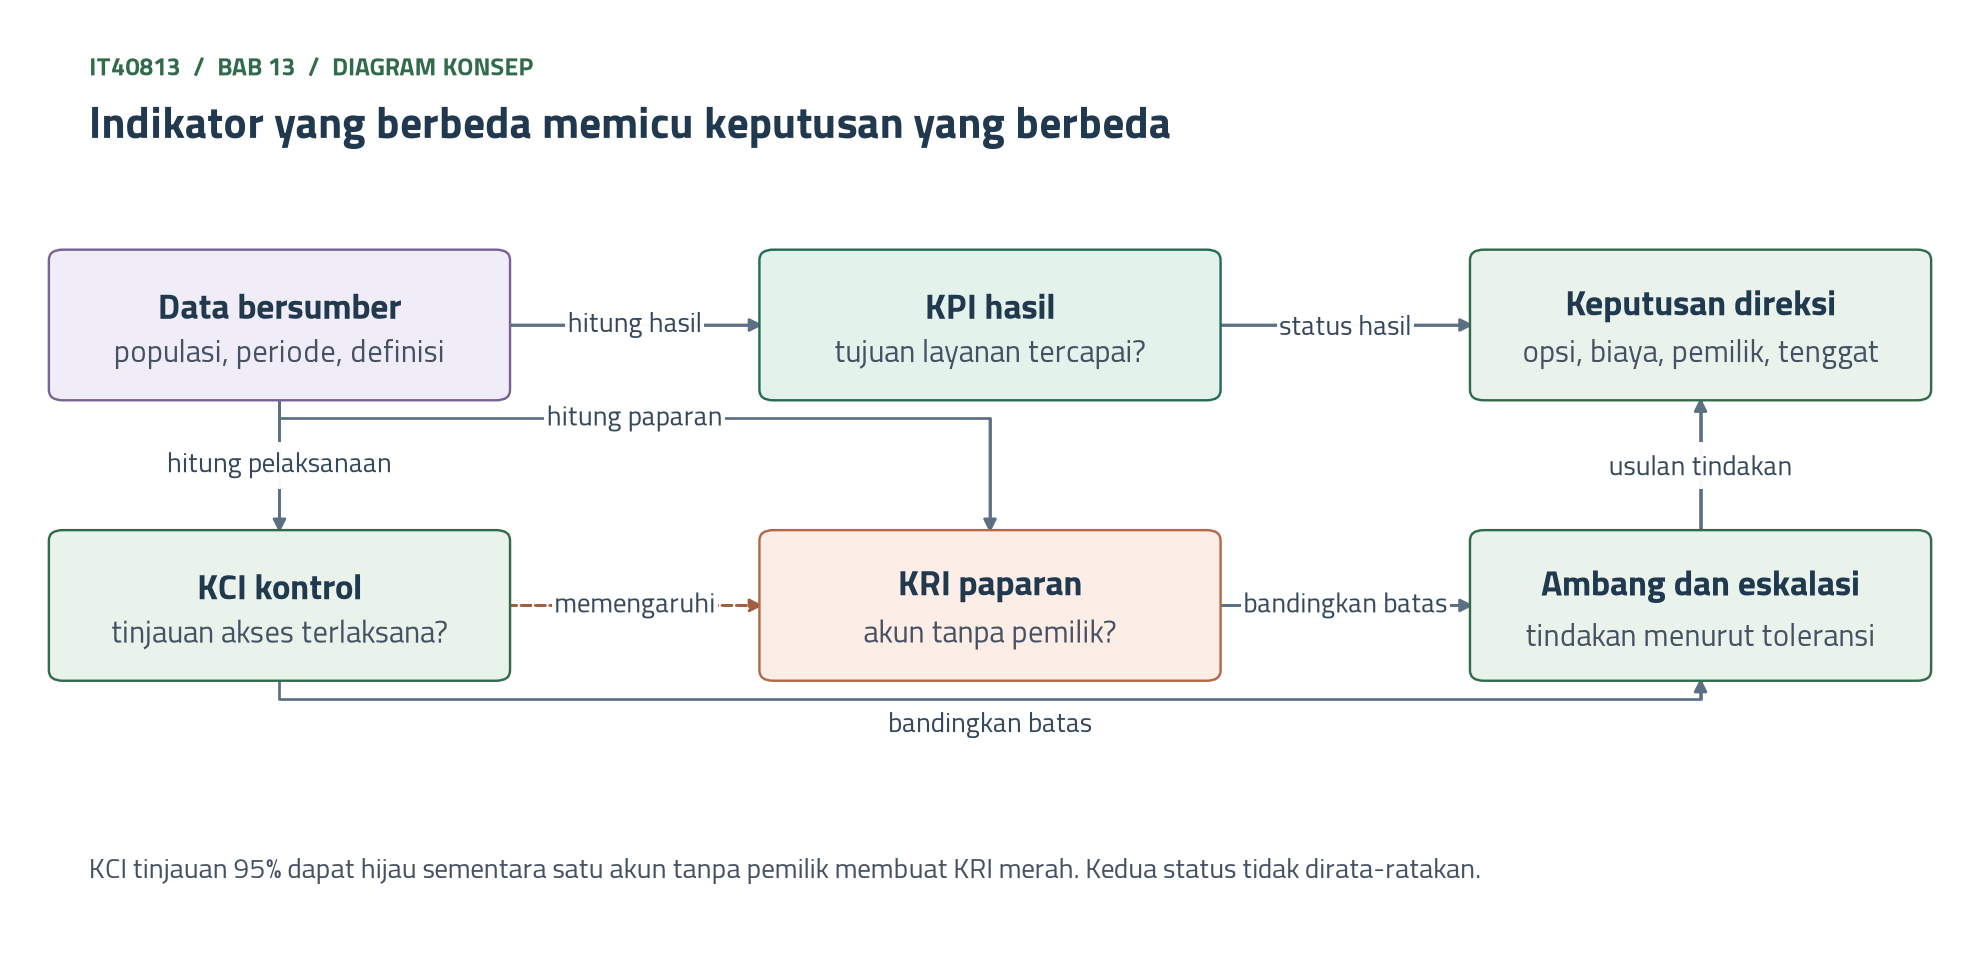
\includegraphics[width=0.96\textwidth,height=0.77\textheight,keepaspectratio]{../../figures/ch13-diagram-konsep.png}
  \label{fig:session13-ilustrasi-bab}
\end{frame}

\section{KPI, KRI, dan KCI}

\begin{frame}{{\Large Tiga Pertanyaan yang Berbeda}}
  \vspace{4pt}
  \footnotesize
  \begin{tabularx}{\textwidth}{|>{\raggedright\arraybackslash}p{0.08\textwidth}|>{\raggedright\arraybackslash}p{0.23\textwidth}|>{\raggedright\arraybackslash}X|>{\raggedright\arraybackslash}X|}
    \hline
    \textbf{Jenis} & \textbf{Pertanyaan} & \textbf{Ukuran contoh} & \textbf{Keputusan yang
    dipicu} \\ \hline
    KPI & Apakah hasil tercapai? & Waktu tunggu 28 menit, target 25 menit & Alur dan jadwal
    petugas diubah atau dipertahankan? \\ \hline
    KRI & Apakah paparan mendekati batas? & 1 akun vendor tanpa pemilik, batas 0 & Akun dibekukan
    atau diberi pengecualian? \\ \hline
    KCI & Apakah kontrol dijalankan? & 114 dari 120 akun ditinjau tepat waktu & Daftar diperbaiki
    atau peninjau ditambah? \\ \hline
  \end{tabularx}

  \vspace{8pt}
  \small Analogi kendaraan pengantar obat: waktu tiba menunjukkan hasil, suhu mesin menunjukkan
  potensi gangguan, dan buku servis menunjukkan pelaksanaan kontrol. KCI mengukur pekerjaan
  organisasi, sedangkan KRI mengukur keadaan yang dihadapi.
\end{frame}

\begin{frame}{{\Large KCI Memengaruhi KRI: Hitungan R-01}}
  \vspace{4pt}
  \footnotesize
  \begin{tabularx}{\textwidth}{|>{\raggedright\arraybackslash}X|>{\raggedright\arraybackslash}p{0.2\textwidth}|>{\raggedright\arraybackslash}p{0.22\textwidth}|>{\raggedright\arraybackslash}p{0.22\textwidth}|}
    \hline
    \textbf{Cakupan AC-01} & \textbf{Peluang R-01} & \textbf{Harapan kerugian} & \textbf{Peluang
    rugi Rp1,5 miliar atau lebih} \\ \hline
    85 persen (Agustus) & 0,0725 & Rp36,25 juta & 1,45 persen \\ \hline
    90 persen (September) & 0,065 & Rp32,5 juta & 1,3 persen \\ \hline
    95 persen (Oktober) & 0,0575 & Rp28,75 juta & 1,15 persen \\ \hline
    100 persen (sasaran) & 0,05 & Rp25 juta & 1 persen \\ \hline
  \end{tabularx}

  \vspace{8pt}
  \small Pengandaian kasar Bab 5: peluang $= 0{,}2 - 0{,}15 \times$ cakupan. Hubungan ini bukan
  hukum sebab akibat. Kewajiban nol akun tanpa pemilik tetap berlaku walaupun selisih 5 persen
  terakhir hanya Rp3,75 juta per tahun.
\end{frame}

\begin{frame}{{\Large Mendahului dan Tertinggal}}
  \vspace{6pt}
  \small
  \begin{itemize}
    \item COSO menelusuri mundur: kejadian risiko, kejadian antara, lalu akar penyebab.
    \item Analogi banjir: air di bendungan hulu memberi waktu mengungsi. Rumah terendam hanya
          menghitung akibat.
    \item Mendahului: akun lewat masa berlaku naik dari 1 menjadi 5 memicu pemeriksaan (Bab 5).
    \item Tertinggal: pemberitahuan hanya bernilai bila ada insiden wajib.
    \item KRI tidak mengelola risiko. Rancangan buruk memberi rasa aman palsu.
  \end{itemize}
\end{frame}

\begin{frame}{{\Large Rantai Kejadian R-01}}
  \vspace{4pt}
  \begin{center}
    \resizebox{0.92\textwidth}{!}{\begin{tikzpicture}[node distance=4.5mm, tahap/.style={draw, rounded corners, align=center, text width=2.4cm, minimum height=1.5cm, font=\scriptsize}, ukur/.style={draw, align=center, text width=2.4cm, minimum height=1.25cm, font=\scriptsize, fill=blue!8}, panah/.style={-{Stealth[length=2mm]}, thick}]
  \node[tahap,fill=blue!8] (a) {\textbf{Akar penyebab}\\[1pt]{\tiny\mdseries tanggal berakhir tidak masuk daftar}};
  \node[tahap,fill=orange!12] (b) [right=of a] {\textbf{Kejadian antara}\\[1pt]{\tiny\mdseries akun aktif melewati masa berlaku}};
  \node[tahap,fill=red!22] (c) [right=of b] {\textbf{Kejadian risiko}\\[1pt]{\tiny\mdseries akun membaca data pasien tanpa tugas}};
  \node[tahap,fill=gray!35] (d) [right=of c] {\textbf{Akibat}\\[1pt]{\tiny\mdseries pemberitahuan dan kerugian}};
  \draw[panah] (a) -- (b);
  \draw[panah] (b) -- (c);
  \draw[panah] (c) -- (d);
  \node[ukur] (ua) [below=6mm of a] {\textbf{KCI IK-07}\\{\tiny\mdseries cakupan peninjauan AC-01}};
  \node[ukur] (ub) [below=6mm of b] {\textbf{KRI IK-01, IK-02}\\{\tiny\mdseries akun tanpa pemilik; lewat masa berlaku}};
  \node[ukur] (uc) [below=6mm of c] {\textbf{Tinjauan \textit{log}}\\{\tiny\mdseries 247 dari 260 tinjauan mingguan (Bab 8)}};
  \node[ukur] (ud) [below=6mm of d] {\textbf{KPI IK-11}\\{\tiny\mdseries pemberitahuan tepat waktu}};
  \draw[-, dashed] (a) -- (ua);
  \draw[-, dashed] (b) -- (ub);
  \draw[-, dashed] (c) -- (uc);
  \draw[-, dashed] (d) -- (ud);
  \draw[panah] ([yshift=-5mm]ua.south west) -- node[below, font=\scriptsize] {sinyal makin terlambat, waktu untuk bertindak makin pendek} ([yshift=-5mm]ud.south east);
\end{tikzpicture}
}
  \end{center}
\end{frame}

\begin{frame}{{\Large Pemeriksaan Keseimbangan}}
  \vspace{4pt}
  \footnotesize
  \begin{tabularx}{\textwidth}{|>{\raggedright\arraybackslash}p{0.19\textwidth}|>{\raggedright\arraybackslash}X|>{\raggedright\arraybackslash}p{0.14\textwidth}|>{\raggedright\arraybackslash}p{0.27\textwidth}|}
    \hline
    \textbf{Perspektif} & \textbf{Pertanyaan} & \textbf{Indikator} & \textbf{Oktober 2026} \\ \hline
    Keuangan & Peluang kerugian besar di dalam batas? & IK-04 & 1 skenario di atas 2 persen \\
    \hline
    Pasien & Layanan lebih cepat dan tersedia? & IK-03, IK-12 & 100 menit gangguan; tunggu 28
    menit \\ \hline
    Proses internal & Kontrol berjalan dan bekerja? & IK-07, IK-08 & Cakupan 95 persen; 10 dari
    12 uji lulus \\ \hline
    Pembelajaran & Temuan menghasilkan perbaikan? & IK-10 & 9 dari 10 tertutup \\ \hline
  \end{tabularx}

  \vspace{8pt}
  \small Balanced Scorecard (Kaplan dan Norton, 1992) dipakai sebagai pemeriksaan keseimbangan,
  bukan sebagai sistem manajemen. Bab 2: kemajuan pekerjaan 90 persen, capaian manfaat 13,3
  persen.
\end{frame}

\section{Merancang Indikator}

\begin{frame}{{\Large Indikator yang Baik Menurut NIST}}
  \vspace{6pt}
  \small
  \begin{itemize}
    \item Penilaian menimbang terhadap kriteria. Pengukuran menghasilkan nilai kuantitatif.
    \item Metrik melacak kemajuan, membantu keputusan, dan memperbaiki kinerja terhadap sasaran.
    \item Sifatnya objektif, akurat, presisi, terikat titik waktu, dapat diulang, dan sebanding.
    \item Empat jenis ukuran: implementasi, efektivitas, efisiensi, dan dampak.
    \item Analogi nilai kelas: rata-rata 90 berbeda bila hanya menghitung siswa yang hadir.
  \end{itemize}
\end{frame}

\begin{frame}{{\Large Kartu Definisi IK-07 (Misalkan)}}
  \vspace{2pt}
  \scriptsize
  \begin{tabularx}{\textwidth}{|>{\raggedright\arraybackslash}p{0.24\textwidth}|>{\raggedright\arraybackslash}X|}
    \hline
    \textbf{Unsur} & \textbf{Isi} \\ \hline
    Pembilang & Akun aktif yang ditinjau dalam bulan berjalan, dengan tanggal bukti \\ \hline
    Penyebut & Semua akun aktif pada daftar penugasan: 120 akun pada 5 rumah sakit \\ \hline
    Sumber & Daftar penugasan dan catatan peninjauan, bukan daftar dari sistem yang diperiksa \\
    \hline
    Frekuensi & Bulanan; ekstrak pada hari kerja terakhir, versi disimpan \\ \hline
    Pemilik dan penerima & Kepala operasi TI; pemilik Medikara+ sebagai pemilik R-01 \\ \hline
    Ambang & Minimal 95 persen hijau; 90 sampai kurang dari 95 kuning; kurang dari 90 merah \\
    \hline
    Tindakan & Periksa kelengkapan daftar; koreksi kuning 5 hari kerja; merah dieskalasi \\ \hline
    Pemeriksa mutu & Audit internal mencocokkan sampel 30 akun (Bab 12) \\ \hline
  \end{tabularx}
\end{frame}

\begin{frame}{{\Large Penyebut Menentukan Cerita}}
  \vspace{6pt}
  \small
  \begin{itemize}
    \item Laporan unit TI: 108 dari 108 akun, atau 100 persen.
    \item Penyebut yang benar: $108 / 120 = 90$ persen. Sebanyak 12 akun tidak pernah ditinjau.
    \item Misalkan sesudah perbaikan, pembilang diperketat menjadi tepat waktu dalam bulan itu.
    \item Agustus: $102 / 120 = 85$ persen. Angka turun karena definisi lebih ketat.
    \item Perubahan definisi dicatat. Tren lama tidak disambung tanpa catatan.
  \end{itemize}
\end{frame}

\begin{frame}{{\Large Nol, Tidak Berlaku, dan Data Tidak Tersedia}}
  \vspace{4pt}
  \footnotesize
  \begin{tabularx}{\textwidth}{|>{\raggedright\arraybackslash}p{0.22\textwidth}|>{\raggedright\arraybackslash}X|>{\raggedright\arraybackslash}p{0.28\textwidth}|}
    \hline
    \textbf{Keadaan} & \textbf{Contoh} & \textbf{Status} \\ \hline
    Nol yang sah & 0 baris kewajiban lewat tenggat, register lengkap & Dinilai: hijau \\ \hline
    Tidak berlaku & 0 pemberitahuan wajib, sehingga penyebut nol & Bukan 100 persen \\ \hline
    Data tidak tersedia & Ekstrak Bogor gagal, 20 dari 120 akun tidak terbaca & Bukan hijau \\
    \hline
  \end{tabularx}

  \vspace{8pt}
  \small Ketepatan pemberitahuan tiga bulan adalah 1 dari 1, bukan 3 dari 3. Bila ekstrak Bogor
  gagal, ``nol akun tanpa pemilik'' hanya mencakup 100 dari 120 akun, atau 83,3 persen.
\end{frame}

\section{Ambang dan Eskalasi}

\begin{frame}{{\Large Lima Batas Bab 5 Menjadi Ambang KRI}}
  \vspace{2pt}
  \scriptsize
  \begin{tabularx}{\textwidth}{|>{\raggedright\arraybackslash}X|>{\raggedright\arraybackslash}p{0.13\textwidth}|>{\raggedright\arraybackslash}p{0.27\textwidth}|>{\raggedright\arraybackslash}p{0.23\textwidth}|}
    \hline
    \textbf{Batas Bab 5} & \textbf{KRI} & \textbf{Ambang} & \textbf{Tindakan} \\ \hline
    Kerahasiaan: nol akun vendor tanpa pemilik dan masa berlaku & IK-01, IK-02 & 0 hijau; lebih
    dari 0 merah & Validasi 1 hari kerja, bekukan \\ \hline
    Kelangsungan: pendaftaran terganggu paling lama 2 jam per bulan & IK-03 & Sampai 90 menit
    hijau; sampai 120 kuning; di atasnya merah & Siapkan perbaikan; tinjauan mingguan \\ \hline
    Finansial: peluang kerugian Rp1,5 miliar atau lebih paling tinggi 2 persen & IK-04 & 0
    skenario hijau; lebih dari 0 merah & Laporkan ke komite \\ \hline
    Kepatuhan: nol baris K-01 sampai K-16 lewat tenggat tanpa keputusan & IK-05 & 0 hijau; lebih
    dari 0 merah & Catat penyimpangan \\ \hline
    Keselamatan: risiko cedera berat ditinjau dalam 1 hari kerja & IK-06 & 0 terlambat hijau;
    lebih dari 0 merah & Libatkan pimpinan klinis \\ \hline
  \end{tabularx}
\end{frame}

\begin{frame}{{\Large Zona Ambang IK-03}}
  \vspace{4pt}
  \begin{center}
    \resizebox{0.85\textwidth}{!}{\begin{tikzpicture}[x=0.062cm, y=1cm, panah/.style={-{Stealth[length=2mm]}, thick}, zona/.style={draw, minimum height=0.8cm, font=\scriptsize\bfseries}, titik/.style={circle, fill=black, inner sep=1.6pt}]
  % Zona dibaca dari batas Bab 5 dan RTO Bab 10, satu satuan x sama dengan satu menit.
  \fill[green!10] (0,0) rectangle (90,0.8);
  \fill[orange!12] (90,0) rectangle (120,0.8);
  \fill[red!22] (120,0) rectangle (180,0.8);
  \draw (0,0) rectangle (180,0.8);
  \draw (90,0) -- (90,0.8);
  \draw (120,0) -- (120,0.8);
  \node[font=\scriptsize\bfseries] at (45,0.4) {Hijau};
  \node[font=\scriptsize\bfseries] at (105,0.4) {Kuning};
  \node[font=\scriptsize\bfseries] at (150,0.4) {Merah};
  \draw[panah] (0,-0.08) -- (186,-0.08) node[right, font=\scriptsize] {menit};
  \foreach \menit in {0,90,120,180} {
    \draw (\menit,-0.14) -- (\menit,-0.02);
    \node[below, font=\scriptsize] at (\menit,-0.14) {\menit};
  }
  \node[below, align=center, text width=2.5cm, font=\tiny] at (82,-0.48) {RTO pendaftaran\\(Bab 10)};
  \node[below, align=center, text width=2.5cm, font=\tiny] at (128,-0.48) {Batas 2 jam per bulan\\(Bab 5)};
  \node[titik] (ags) at (150,0.8) {};
  \node[titik] (sep) at (40,0.8) {};
  \node[titik] (okt) at (100,0.8) {};
  \node[above, align=center, font=\scriptsize] at (ags.north) {Agustus\\150};
  \node[above, align=center, font=\scriptsize] at (sep.north) {September\\40};
  \node[above, align=center, font=\scriptsize] at (okt.north) {Oktober\\100};
\end{tikzpicture}
}
  \end{center}
  \vspace{2pt}
  \small Satu kejadian yang memenuhi RTO 90 menit menyisakan 30 menit. Rata-rata tiga bulan 96,7
  menit menyembunyikan pelanggaran Agustus, karena batas Bab 5 berbunyi per bulan.
\end{frame}

\begin{frame}{{\Large Toleransi Nol dan Aturan Tepi}}
  \vspace{6pt}
  \small
  \begin{itemize}
    \item Tren 3, 2, 1 tetap merah sampai nol. Zona kuning buatan melunakkan batas.
    \item Peringatan dini berpindah ke IK-02 dan IK-07.
    \item Pengecualian darurat dicatat terpisah. Sesudah 24 jam, akun masuk hitungan IK-01.
    \item Status memakai nilai sebelum pembulatan: $113 / 120 = 94{,}17$ persen berstatus kuning.
    \item Populasi kecil: 5 DPIA berarti satu butir 20 persen, sehingga ambang kuning 80 persen.
  \end{itemize}
\end{frame}

\begin{frame}{{\Large Jalur Eskalasi Memakai Batas Delegasi Bab 2}}
  \vspace{2pt}
  \scriptsize
  \begin{tabularx}{\textwidth}{|>{\raggedright\arraybackslash}p{0.21\textwidth}|>{\raggedright\arraybackslash}X|>{\raggedright\arraybackslash}p{0.3\textwidth}|}
    \hline
    \textbf{Tingkat} & \textbf{Pemicu} & \textbf{Waktu} \\ \hline
    Pemilik tindakan & Nilai kuning atau merah & Merah 1 hari kerja; kuning 5 hari kerja \\ \hline
    Pemilik risiko & Merah belum tertutup; butuh pengecualian & Hari kerja berikutnya; pengecualian
    paling lama 24 jam \\ \hline
    Kepala TI & Biaya sampai Rp100 juta & Ringkasan triwulan ke komite \\ \hline
    Komite pengarah TI & Di atas Rp100 juta sampai Rp400 juta; merah dua bulan berturut-turut &
    Rapat bulanan \\ \hline
    Direksi & Di atas Rp400 juta sampai Rp5 miliar; penerimaan risiko di atas batas & Triwulan,
    atau segera bila pemicu krisis organisasi terpenuhi \\ \hline
    Dewan komisaris & Di atas Rp5 miliar, bila anggaran dasar menetapkan & Laporan triwulan \\
    \hline
  \end{tabularx}

  \vspace{6pt}
  IK-06 langsung melibatkan pimpinan klinis. Pemberitahuan K-04 mengikuti jam insiden Bab 7.
\end{frame}

\begin{frame}{{\Large Kasus Medikara: Satu Akun pada Oktober}}
  \vspace{6pt}
  \small
  \begin{itemize}
    \item Misalkan ekstrak Oktober menemukan 1 akun tanpa pemilik, divalidasi dalam 1 hari kerja.
    \item Pemilik Medikara+ membekukan akun dan menolak pengecualian 24 jam.
    \item Biaya: pekerjaan teknisi tertunda 1 hari kerja.
    \item IK-01 tetap merah pada laporan, karena nilainya keadaan pada tanggal data.
    \item Rekonsiliasi sampai Rp60 juta di bawah batas Rp100 juta: kepala TI yang memutuskan.
  \end{itemize}
\end{frame}

\section{Portofolio Metrik}

\begin{frame}{{\Large Memilih dari Pertanyaan, Bukan dari Data}}
  \vspace{6pt}
  \small
  \begin{itemize}
    \item NIST: metrik yang salah pilih merusak mutu laporan. Pada tahap awal, lebih sedikit
          sering lebih baik.
    \item Uji: apakah data menggambarkan kinerja kontrol, atau melacak risiko yang material?
    \item Analogi pemeriksaan kesehatan: tiap angka punya batas dan tindak lanjut.
    \item Kasus: 46 usulan, 19 gugur, 15 tingkat operasional, 12 indikator.
    \item CSF GV.OV-03: kinerja pengelolaan risiko dievaluasi dan ditinjau untuk penyesuaian.
  \end{itemize}
\end{frame}

\begin{frame}{{\Large Portofolio Dua Belas Indikator (Misalkan)}}
  \vspace{0pt}
  \fontsize{7}{8.5}\selectfont
  \renewcommand{\arraystretch}{1.02}
  \begin{tabularx}{\textwidth}{|>{\raggedright\arraybackslash}p{0.07\textwidth}|>{\raggedright\arraybackslash}X|>{\raggedright\arraybackslash}p{0.06\textwidth}|>{\raggedright\arraybackslash}p{0.2\textwidth}|>{\raggedright\arraybackslash}p{0.17\textwidth}|}
    \hline
    \textbf{Kode} & \textbf{Indikator} & \textbf{Jenis} & \textbf{Pemilik tindakan} &
    \textbf{Kaitan} \\ \hline
    IK-01 & Akun vendor aktif tanpa pemilik atau masa berlaku & KRI & Kepala operasi TI & R-01,
    AC-01 \\ \hline
    IK-02 & Akun melewati masa berlaku & KRI & Kepala operasi TI & R-01, AC-01 \\ \hline
    IK-03 & Menit gangguan pendaftaran & KRI & Kepala operasi TI & R-03, R-05 \\ \hline
    IK-04 & Skenario melewati batas peluang kerugian & KRI & Kepala risiko & R-01, R-05 \\ \hline
    IK-05 & Baris kewajiban lewat tenggat tanpa keputusan & KRI & Fungsi kepatuhan & K-01 sampai
    K-16 \\ \hline
    IK-06 & Risiko cedera berat lewat tinjauan 1 hari kerja & KRI & Pimpinan klinis & R-11 \\ \hline
    IK-07 & Cakupan peninjauan AC-01 & KCI & Kepala operasi TI & R-01, AC-01 \\ \hline
    IK-08 & Uji pemulihan lulus, gabungan dan rumah sakit & KCI & Kepala operasi TI & R-05, K-02 \\
    \hline
    IK-09 & DPIA selesai & KCI & Petugas pelindungan data & 5 DPIA Bab 7 \\ \hline
    IK-10 & Temuan tertutup tepat waktu sesudah uji ulang & KPI & Pemilik tiap temuan & TA-01 dan
    lainnya \\ \hline
    IK-11 & Pemberitahuan tepat waktu & KPI & Petugas pelindungan data & R-12, K-04 \\ \hline
    IK-12 & Waktu tunggu pendaftaran 18 klinik & KPI & Kepala pendaftaran & Bab 1 dan Bab 2 \\
    \hline
  \end{tabularx}
\end{frame}

\begin{frame}{{\Large Bahan dari Bab 8 sampai Bab 12}}
  \vspace{0pt}
  \tiny
  \begin{tabularx}{\textwidth}{|>{\raggedright\arraybackslash}p{0.07\textwidth}|>{\raggedright\arraybackslash}X|>{\raggedright\arraybackslash}p{0.27\textwidth}|>{\raggedright\arraybackslash}p{0.16\textwidth}|}
    \hline
    \textbf{Asal} & \textbf{Bahan} & \textbf{Diolah menjadi} & \textbf{Pembaca} \\ \hline
    Bab 8 & T-19: 247 dari 260 tinjauan \textit{log} mingguan, 95 persen & KCI jejak aktivitas &
    Komite pengarah TI \\ \hline
    Bab 9 & Akun vendor tanpa pemilik, 0 akun & IK-01 & Direksi bila merah \\ \hline
    Bab 9 & Catatan AC-01, 60 dari 60 per tahun atau 5 per bulan & Rincian IK-07 & Pemilik risiko
    \\ \hline
    Bab 9 & Laporan dugaan insiden vendor 12 jam, K-05 & Masuk IK-05 bila lewat tenggat tanpa
    keputusan & Komite risiko \\ \hline
    Bab 9 & Latihan bersama 2 per tahun; subprosesor 30 hari; uji ekspor 1 per tahun & Kalender
    kontrol & Pengelola vendor \\ \hline
    Bab 10 & RTO 90 menit; 29 dari 36 uji; 3 dari 5 rumah sakit & IK-03, IK-08 & Direksi \\ \hline
    Bab 11 & 27 dari 30 kasus darurat tertangkap; 93 dari 120 tanda klinik keliru; AI-03 selisih
    8, ambang 5 & KCI mutu AI; jalur penyebab R-11 pada IK-06, tanpa kode baru & Komite risiko \\
    \hline
    Bab 12 & TA-01; 24 dari 30 akun sesuai; kriteria 30 dari 30 & IK-10; pemeriksa mutu IK-07 &
    Direksi bila lewat tenggat \\ \hline
  \end{tabularx}

  \vspace{6pt}
  \scriptsize SLO disinggung saja. Layanan pesan 99,5 persen dari 8.760 jam dan batas pendaftaran
  24 jam dari 4.380 jam memiliki dasar hitung berbeda, sehingga tidak digabung.
\end{frame}

\section{Mutu Data dan Manipulasi}

\begin{frame}{{\Large Sumber Data dan Mutu Data}}
  \vspace{6pt}
  \small
  \begin{itemize}
    \item NIST: validitas diragukan bila sumber hanya memuat sebagian unit atau proses tidak
          konsisten.
    \item COSO: tanpa keseragaman cara ukur, data gabungan menambah gangguan pada keputusan.
    \item Analogi timbangan pasar: harga antarkios tidak sebanding bila timbangan berbeda.
    \item Laporan 18 klinik: 2 jam per klinik per bulan menjadi 432 jam per tahun, Rp25,92 juta.
    \item R-04: versi spreadsheet berbeda, harapan kerugian Rp30 juta per tahun.
  \end{itemize}
\end{frame}

\begin{frame}{{\Large Indikator yang Dimanipulasi}}
  \vspace{2pt}
  \scriptsize
  \begin{tabularx}{\textwidth}{|>{\raggedright\arraybackslash}p{0.21\textwidth}|>{\raggedright\arraybackslash}X|>{\raggedright\arraybackslash}X|}
    \hline
    \textbf{Bentuk} & \textbf{Contoh} & \textbf{Pengaman} \\ \hline
    Mengecilkan penyebut & 12 akun keluar dari daftar, 90 menjadi 100 persen & Populasi dari daftar
    penugasan \\ \hline
    Memindahkan kategori & Insiden wajib dicatat tidak wajib & Alasan ditinjau fungsi hukum \\
    \hline
    Menutup di atas kertas & Selesai menurut manajemen: 100 persen; lolos uji ulang: 90 persen &
    Hitung sesudah uji ulang \\ \hline
    Mengejar batas & Peninjauan tergesa supaya tepat 95 persen & Sampel mutu; catatan per akun \\
    \hline
    Mengubah definisi & Tepat waktu digeser dari 30 menjadi 45 hari & Riwayat definisi; tren tidak
    disambung \\ \hline
  \end{tabularx}

  \vspace{6pt}
  \small Bevan dan Hood (2006): tata kelola lewat target mengandaikan bagian mewakili keseluruhan,
  serta masalah pengukuran dan \textit{gaming} tidak penting. Contoh: 125 menit gangguan menjadi 85
  menit karena 40 menit disebut pemeliharaan.
\end{frame}

\section{Dashboard}

\begin{frame}{{\Large Dashboard: Keadaan, Tren, dan Pengecualian}}
  \vspace{6pt}
  \small
  \begin{itemize}
    \item Few: informasi terpenting pada satu layar, dapat dipantau sekilas.
    \item \textit{Dashboard} memberi tahu apa yang terjadi, bukan mengapa.
    \item Analogi papan keberangkatan: kereta, jam, dan status. Alasan dicari di tempat lain.
    \item Warna selalu disertai angka dan kata status. Pengecualian ditaruh lebih dahulu.
    \item Tiga nilai terakhir terlihat. Perubahan definisi diberi catatan.
  \end{itemize}
\end{frame}

\begin{frame}{{\Large Dashboard GRC, Oktober 2026 (Misalkan)}}
  \vspace{-2pt}
  \begin{center}
    \resizebox{!}{0.72\textheight}{\begin{tikzpicture}[petak/.style={draw, rounded corners=1pt, align=center, text width=2.55cm, minimum height=2.05cm, font=\scriptsize, execute at begin node={\hyphenpenalty=10000}}]
  % Baris disusun dari pengecualian: merah lebih dahulu, lalu kuning, hijau, dan tidak berlaku.
  \node[petak,fill=red!22] at (0,0) {\textbf{IK-01 Akun tanpa pemilik}\\{\footnotesize\textbf{1 akun}}\\MERAH\\{\tiny\mdseries 3, 2, 1}};
  \node[petak,fill=red!22] at (2.85,0) {\textbf{IK-04 Skenario lewat batas}\\{\footnotesize\textbf{1 (R-05)}}\\MERAH\\{\tiny\mdseries 1, 1, 1}};
  \node[petak,fill=red!22] at (5.7,0) {\textbf{IK-08 Uji pemulihan}\\{\footnotesize\textbf{83,3\%}}\\MERAH\\{\tiny\mdseries rumah sakit 1 dari 2}\\{\tiny\mdseries 75\%, 83,3\%, 83,3\%}};
  \node[petak,fill=orange!12] at (8.55,0) {\textbf{IK-03 Gangguan pendaftaran}\\{\footnotesize\textbf{100 menit}}\\KUNING\\{\tiny\mdseries 150, 40, 100}};
  \node[petak,fill=orange!12] at (0,-2.15) {\textbf{IK-12 Waktu tunggu}\\{\footnotesize\textbf{28 menit}}\\KUNING\\{\tiny\mdseries 34, 31, 28}};
  \node[petak,fill=green!10] at (2.85,-2.15) {\textbf{IK-02 Lewat masa berlaku}\\{\footnotesize\textbf{0 akun}}\\HIJAU\\{\tiny\mdseries 2, 1, 0}};
  \node[petak,fill=green!10] at (5.7,-2.15) {\textbf{IK-05 Kewajiban lewat tenggat}\\{\footnotesize\textbf{0 baris}}\\HIJAU\\{\tiny\mdseries 2, 1, 0}};
  \node[petak,fill=green!10] at (8.55,-2.15) {\textbf{IK-06 Cedera lewat tinjauan}\\{\footnotesize\textbf{0 laporan}}\\HIJAU\\{\tiny\mdseries 0, 1, 0}};
  \node[petak,fill=green!10] at (0,-4.3) {\textbf{IK-07 Cakupan AC-01}\\{\footnotesize\textbf{95\%}}\\HIJAU\\{\tiny\mdseries 85\%, 90\%, 95\%}};
  \node[petak,fill=green!10] at (2.85,-4.3) {\textbf{IK-09 DPIA selesai}\\{\footnotesize\textbf{100\%}}\\HIJAU\\{\tiny\mdseries 60\%, 80\%, 100\%}};
  \node[petak,fill=green!10] at (5.7,-4.3) {\textbf{IK-10 Temuan tertutup}\\{\footnotesize\textbf{90\%}}\\HIJAU\\{\tiny\mdseries 60\%, 80\%, 90\%}};
  \node[petak,fill=gray!35] at (8.55,-4.3) {\textbf{IK-11 Pemberitahuan}\\{\footnotesize\textbf{Nol kewajiban}}\\TIDAK BERLAKU\\{\tiny\mdseries 100\%, lalu tidak berlaku}};
\end{tikzpicture}
}
  \end{center}
\end{frame}

\begin{frame}{{\Large Tren Dua Belas Indikator (Misalkan)}}
  \vspace{0pt}
  \tiny
  \begin{tabularx}{\textwidth}{|>{\raggedright\arraybackslash}X|>{\raggedright\arraybackslash}p{0.24\textwidth}|>{\raggedright\arraybackslash}p{0.24\textwidth}|>{\raggedright\arraybackslash}p{0.24\textwidth}|}
    \hline
    \textbf{Indikator} & \textbf{Agustus} & \textbf{September} & \textbf{Oktober} \\ \hline
    IK-01 Akun tanpa pemilik & 3, merah & 2, merah & 1, merah \\ \hline
    IK-02 Lewat masa berlaku & 2, merah & 1, merah & 0, hijau \\ \hline
    IK-03 Gangguan pendaftaran & 150 menit, merah & 40 menit, hijau & 100 menit, kuning \\ \hline
    IK-04 Skenario lewat batas & 1, merah & 1, merah & 1, merah \\ \hline
    IK-05 Kewajiban lewat tenggat & 2, merah & 1, merah & 0, hijau \\ \hline
    IK-06 Cedera lewat tinjauan & 0, hijau & 1, merah & 0, hijau \\ \hline
    IK-07 Cakupan AC-01 & 102/120 = 85\%, merah & 108/120 = 90\%, kuning & 114/120 = 95\%, hijau
    \\ \hline
    IK-08 Uji pemulihan & 9/12 = 75\%; rumah sakit 1/2, merah & 10/12 = 83,33\%; 1/1, kuning &
    10/12 = 83,33\%; 1/2, merah \\ \hline
    IK-09 DPIA selesai & 3/5 = 60\%, merah & 4/5 = 80\%, kuning & 5/5 = 100\%, hijau \\ \hline
    IK-10 Temuan tertutup & 6/10 = 60\%, merah & 8/10 = 80\%, kuning & 9/10 = 90\%, hijau \\ \hline
    IK-11 Pemberitahuan & 1/1 = 100\%, hijau & Tidak berlaku & Tidak berlaku \\ \hline
    IK-12 Waktu tunggu & 34 menit, merah & 31 menit, merah & 28 menit, kuning \\ \hline
  \end{tabularx}
\end{frame}

\begin{frame}{{\Large Mengapa Tanpa Skor Gabungan}}
  \vspace{6pt}
  \small
  \begin{itemize}
    \item Misalkan hijau 100, kuning 50, merah 0, dan tidak berlaku dikeluarkan.
    \item Skor gabungan: 16,7, lalu 27,3, lalu $700 \div 11 \approx 63{,}6$.
    \item Skor naik hampir empat kali lipat, sementara IK-01 dan IK-04 merah pada ketiga bulan.
    \item Hijau dan merah tidak dirata-ratakan menjadi kuning.
    \item Harganya: satu baris lebih untuk tiap pengecualian, tanpa satu angka yang mudah diingat.
  \end{itemize}
\end{frame}

\section{Laporan ke Direksi}

\begin{frame}{{\Large Struktur Laporan Satu Halaman}}
  \vspace{-2pt}
  \begin{center}
    \resizebox{!}{0.72\textheight}{\begin{tikzpicture}[blok/.style={draw, align=left, text width=7.1cm, font=\scriptsize, inner sep=3pt}, catatan/.style={align=left, text width=3.5cm, font=\scriptsize, execute at begin node={\hyphenpenalty=10000}}, panah/.style={-{Stealth[length=2mm]}, thick}]
  \node[blok,fill=praditagreen!15] (kepala) {\textbf{Laporan GRC Triwulan Agustus sampai Oktober 2026}\\{\tiny\mdseries Cakupan, tanggal data, penyusun, dan pemilik laporan}};
  \node[blok,fill=orange!12,below=1.5mm of kepala] (putus) {\textbf{Keputusan yang diminta}\\{\tiny\mdseries Setujui, ubah, atau tolak: tahap kedua Rp180 juta untuk opsi B, paling lambat akhir November 2026}};
  \node[blok,fill=blue!8,below=1.5mm of putus] (p1) {\textbf{Pesan 1: Pemulihan belum memenuhi syarat}\\{\tiny\mdseries 3 dari 5 rumah sakit lulus; R-05 masih 10 persen, batasnya 2 persen}};
  \node[blok,fill=blue!8,below=1mm of p1] (p2) {\textbf{Pesan 2: Akses vendor membaik, belum selesai}\\{\tiny\mdseries Cakupan 95 persen; 1 akun tanpa pemilik dibekukan; TA-01 belum tertutup}};
  \node[blok,fill=blue!8,below=1mm of p2] (p3) {\textbf{Pesan 3: Layanan membaik, masih di bawah target}\\{\tiny\mdseries Waktu tunggu 34, 31, 28 menit; gangguan 150, 40, 100 menit}};
  \node[blok,fill=blue!8,below=1.5mm of p3] (opsi) {\textbf{Tabel tiga pilihan}\\{\tiny\mdseries Biaya, akibat pada risiko, pemilik, tenggat, dan ukuran keberhasilan}};
  \node[blok,fill=green!10,below=1.5mm of opsi] (batas) {\textbf{Batas data dan tindak lanjut}\\{\tiny\mdseries Tingkat lulus uji bukan peluang R-05; 5 uji rumah sakit tergolong sedikit}};
  \draw (kepala.north west) rectangle (batas.south east);
  \node[catatan,right=4mm of putus] (c1) {Dibaca pertama: direksi tahu apa yang harus diputuskan};
  \node[catatan,right=4mm of p2] (c2) {Tiga pesan: angka, tren, dan risiko; tanpa daftar kegiatan};
  \node[catatan,right=4mm of opsi] (c3) {Ada pembanding, sehingga usulan dapat ditolak};
  \node[catatan,right=4mm of batas] (c4) {Batas klaim mencegah tafsir berlebihan};
  \draw[panah] (c1.west) -- (putus.east);
  \draw[panah] (c2.west) -- (p2.east);
  \draw[panah] (c3.west) -- (opsi.east);
  \draw[panah] (c4.west) -- (batas.east);
\end{tikzpicture}
}
  \end{center}
\end{frame}

\begin{frame}{{\Large Isi dan Alamat Laporan}}
  \vspace{6pt}
  \small
  \begin{itemize}
    \item NIST: ukuran tanpa konteks menimbulkan keraguan. Sebutkan risiko, batas, dan tindakan.
    \item COSO: frekuensi mengikuti pembaca. Direksi membaca yang teragregasi.
    \item Medikara: \textit{dashboard} bulanan ke komite, laporan triwulan ke direksi (Bab 2).
    \item Daftar 7 kegiatan selesai tidak memberi dasar bertindak.
    \item Rp60 juta salah alamat bila dibawa ke direksi. Rp180 juta tahap kedua milik direksi.
  \end{itemize}
\end{frame}

\begin{frame}{{\Large Kasus Medikara: Tiga Pesan}}
  \vspace{6pt}
  \small
  \begin{itemize}
    \item Pesan 1: pemulihan belum memenuhi syarat. 29 dari 36 uji lulus, 3 dari 5 rumah sakit, 2
          data gagal dari 9 uji akun terpisah. R-05 masih 10 persen, batasnya 2 persen.
    \item Pesan 2: akses vendor membaik, belum selesai. Cakupan 85, 90, 95 persen. Satu akun
          dibekukan. TA-01 belum lolos uji ulang.
    \item Pesan 3: layanan membaik, masih di bawah target. Waktu tunggu 34, 31, 28 menit. Gangguan
          Oktober 100 menit, di atas RTO 90 menit.
  \end{itemize}
\end{frame}

\begin{frame}{{\Large Kasus Medikara: Satu Keputusan}}
  \vspace{2pt}
  \scriptsize
  \begin{tabularx}{\textwidth}{|>{\raggedright\arraybackslash}p{0.27\textwidth}|>{\raggedright\arraybackslash}p{0.13\textwidth}|>{\raggedright\arraybackslash}X|>{\raggedright\arraybackslash}X|}
    \hline
    \textbf{Pilihan} & \textbf{Biaya} & \textbf{Akibat pada R-05} & \textbf{Risiko pilihan} \\
    \hline
    1. Tahan tahap kedua; uji ulang 2 rumah sakit dan 9 uji akun terpisah & Rp0 tambahan saat ini
    & Peluang tetap 0,1; sekitar Rp40 juta lebih tinggi per triwulan & Direksi menerima tertulis
    paparan di atas batas selama satu triwulan \\ \hline
    2. Cairkan Rp180 juta sekarang & Rp180 juta & Peluang tetap dicatat 0,1 sampai uji lulus &
    Syarat hilang; uang keluar sebelum bukti \\ \hline
    3. Hentikan opsi B, kembali ke opsi A & Hemat Rp180 juta & SIMRS pulih 480 menit; batas 2
    persen dilanggar & Sudah ditolak pada Bab 10 \\ \hline
  \end{tabularx}

  \vspace{6pt}
  \small Rekomendasi pilihan 1, keputusan paling lambat akhir November 2026. Keberhasilan: 5 dari
  5 rumah sakit di bawah 120 menit, dan 9 dari 9 uji akun terpisah, paling lambat akhir Januari
  2027.
\end{frame}

\begin{frame}{{\Large Beban Laporan Lama dan Rancangan Baru}}
  \vspace{4pt}
  \footnotesize
  \begin{tabularx}{\textwidth}{|>{\raggedright\arraybackslash}X|>{\raggedright\arraybackslash}p{0.3\textwidth}|>{\raggedright\arraybackslash}p{0.3\textwidth}|}
    \hline
    \textbf{Unsur} & \textbf{Laporan 40 halaman} & \textbf{Satu halaman} \\ \hline
    Penyusunan per tahun & $(8 \times 6 + 16) \times 12 = 768$ jam & $12 \times 2 \times 12 + 4
    \times 24 = 384$ jam \\ \hline
    Biaya per tahun & Rp46,08 juta & Rp23,04 juta \\ \hline
    Waktu baca & 80 menit, 12 kali & Sekitar 5 menit, 4 kali \\ \hline
  \end{tabularx}

  \vspace{8pt}
  \small Penghematan 384 jam berarti indikator tidak menambah beban 3.046 jam pada Bab 14. Rincian
  tetap tersedia di \textit{dashboard} dan katalog bagi pihak yang bertugas memakainya.
\end{frame}

\section{Aktivitas dan Penutup}

\begin{frame}{{\Large Aktivitas: Langkah Kerja}}
  \vspace{4pt}
  \small
  \begin{enumerate}
    \item Pilih 8 sampai 12 indikator. Tulis keputusan yang didukung tiap ukuran.
    \item Isi katalog: rumus, sumber, frekuensi, pemilik, serta ambang tiga warna.
    \item Hitung tiga periode. Bedakan nol, tidak berlaku, dan data tidak tersedia.
    \item Susun \textit{dashboard} pada spreadsheet, lalu tulis tiga pesan dan satu keputusan.
    \item Tinjau silang rumus, lalu simulasikan rapat 5 menit.
  \end{enumerate}
\end{frame}

\begin{frame}{{\Large Aktivitas: Peran, Luaran, dan Penilaian}}
  \vspace{6pt}
  \small
  \begin{itemize}
    \item Peran: analis risiko memimpin ambang, anggota bisnis menyusun narasi, analis teknologi
          memeriksa data, pemilik konteks memeriksa kewenangan.
    \item Luaran masuk C4: katalog, \textit{dashboard}, dan laporan satu halaman.
    \item Kriteria: risiko dan keputusan 30 persen; definisi dan hitungan 30 persen; ambang 20
          persen; permintaan keputusan 20 persen.
    \item Berkas: \texttt{sources/chapter13/README.md}.
    \item Opsional: mengotomasi dua indikator ke Metabase atau Grafana.
  \end{itemize}
\end{frame}

\begin{frame}{{\Large Ringkasan}}
  \vspace{6pt}
  \small
  \begin{itemize}
    \item KPI, KRI, dan KCI menjawab hasil, paparan, dan kontrol. Warnanya tidak dirata-ratakan.
    \item Definisi menentukan cerita: 108 dari 108 berbeda dari 108 dari 120.
    \item Ambang diturunkan dari batas Bab 5. Toleransi nol tetap merah sampai nol.
    \item \textit{Dashboard} menunjukkan keadaan dan tren. Laporan mengajukan pilihan.
    \item Indikator berguna ketika mengubah keputusan dan tindakan, bukan ketika memenuhi halaman.
  \end{itemize}
\end{frame}

\begin{frame}{{\Large Latihan}}
  \vspace{4pt}
  \small
  \begin{enumerate}
    \item ``Jumlah pelatihan keamanan yang diselenggarakan'' diusulkan sebagai KRI. Kritisi usulan
          ini dan tawarkan indikator yang lebih baik.
    \item Turunkan ambang KRI untuk risiko kontrol akses dari pernyataan \textit{risk appetite}
          yang dibuat pada Pertemuan 5.
    \item Jelaskan apa yang membuat sebuah laporan direksi berujung pada keputusan, bukan sekadar
          dibaca.
  \end{enumerate}

  \vspace{6pt}
  Contoh terisi dan lembar isian ada pada modul.
\end{frame}

\begin{frame}{{\Large Bacaan dan Berkas Pendukung}}
  \vspace{6pt}
  \small
  \begin{itemize}
    \item \href{https://doi.org/10.6028/NIST.SP.800-55v1}{NIST SP 800-55 Volume 1} dan
          \href{https://doi.org/10.6028/NIST.SP.800-55v2}{Volume 2}
    \item \href{https://doi.org/10.6028/NIST.CSWP.29}{NIST CSF 2.0}
    \item \href{https://www.coso.org/_files/ugd/3059fc_6b2928dffbdf481dbf32971b3e9b9c85.pdf}{COSO:
          Developing Key Risk Indicators}
    \item \href{https://doi.org/10.1111/j.1467-9299.2006.00600.x}{Bevan dan Hood (2006)} dan
          \href{https://www.perceptualedge.com/articles/ie/dashboard_confusion.pdf}{Few (2004)}
    \item \texttt{sources/chapter13/README.md}
  \end{itemize}
\end{frame}

\end{document}
